\documentclass[12pt,a4paper]{article}
\usepackage{graphicx}
\usepackage[utf8]{inputenc}
\usepackage{hyperref}
\usepackage{pgfplots}
\usepackage{mathtools}

\begin{document}
\begin{titlepage}
	\centering
	\includegraphics[width=0.15\textwidth]{utec.png}\par\vspace{1cm}
	{\scshape\LARGE UTEC \par}
	\vspace{1cm}
	{\scshape\Large Procesador MIPS 32\par}
	\vspace{1.5cm}
	{\huge\bfseries Arquitectura de las Computadoras\par}
	\vspace{2cm}
	{\Large\itshape Alejandro Goicochea\par}
	\href{mailto:alejandro.goicochea@utec.edu.pe}{alejandro.goicochea@utec.edu.pe}
	\vfill
	Profesor:\par
	Jorge Gonzales

	\vfill
	{\large \today\par}
\end{titlepage}

\section{Abstract}
In this report we will detail the implementation of a MIPS32 processor in verilog. It will have a reduced set of instructions from the MIPS reference data card found in the following link: \href{https://inst.eecs.berkeley.edu/~cs61c/resources/MIPS_Green_Sheet.pdf}{MIPS Resource Data Sheet} The implemented instructions are the following:\\


\begin{table}[htb]
\begin{center}
\begin{tabular}{|l|l|l|l|}
\hline
add & addi & lb  & beq  \\ \hline
sub & andi & lh  & bneq \\ \hline
and & ori  & lw  & bgez \\ \hline
nor & slti & sb  & j    \\ \hline
or  &      & sh  & jr   \\ \hline
slt &      & sw  & jal  \\ \hline
    &      & lui &      \\ \hline
\end{tabular}
\end{center}
\end{table}

Since the bgez instruction is not specified there, we will use the opcode $000001$ for it.

\section{Introduction}
A procesor is the core of all computers, it is in charge of carrying out all the instructions needed and acts as a sort of "brain" for the computer. Nowadays we have a variety of procesors varying from architecture to processing speed. The processor we will implement is a MIPS32, meaning that it takes 32-bit instructions. The processor will have all the basic hardware it needs, only implementing an l1 cache.



\section{Methodology}
For the implementation of the processor the following modules were used:
\begin{enumerate}
\item DataPath
\item InstructionMemory
\item InstructionProcess
\item Registers
\item DataMemory
\item ALU
\item ControlUnit
\item MemToReg
\end{enumerate}

\subsection{Datapath}
\text This module is the base of the processor, it is in charge of sending information to all the modules through wires and it declares all the registers that will be used such as the signals and registers for all register data. Furthermore, it is in charge of the program counter increments through jumps, branches or the default increment of 4.

\subsection{InstructionMemory}
\text This module stores all the instructions of our program. It opens a text file and stores it in a register. Whenever a $pc$ arrives it sends out a 32-bit instruction back to the datapath, to do this it takes the next four addresses of the instruction register to form the whole instruction since our memory is byte-addressable.

\subsection{InstructionProcess}
\text This module divides the instruction in its different parts depending on the opcode it gets. With the opcode it knows if the instruction is of type $I$, $R$ or $J$.

\subsection{Registers}
\text This module is in charge of the 32 registers that the processor has. It is sepparated in two always blocks, one for writing and the other for reading so it has a signal for each. It also has another signal that determines if the module writes to the address stored in $rt$ or $rd$, depending on the type of instruction it got. If the instruction is of type $I$, it will check the opcode to see if it is a load instruction as a different amount of bits is stored with the different load instructions. The register is loaded incially with $0's$ from a text file and outputs the result into a new file to make sure the program executed correctly.

\subsection{DataMemory}
\text The DataMemory module is in charge of the memory inside the processor. It is loaded from a file containing $0's$ and has two functions: write and read. This module is only called for load and store instructions, sending data to the register file in case of a load instruction and storing it in the memory in case of a store instruction. It uses signals $memWrite$ and $memRead$ to determine what to do with the data it gets.

\subsection{ALU}
\text La ALU module is in charge of all arithmetic operations. It also sends the branch signal to the datapath to know what to do with the program counter. It always checks the opcode first and if the instruction is of type $R$, it checks the $funct$ value to know what opperation to carry out. It also creates signed registers before the operations in order to work with negative numbers correctly where they are needed.

\subsection{ControlUnit}
\text This module is in charge of setting the signals that will be used to control the flow of data inside of our processor. It decides on this depeding on the $opcode$ and funct of the instruction that was fetched by the datapath module. All signals except for $rt_rd$ are inicialized on 0 and swapped accordingly.

\subsection{MemToReg}
\text This module is a 2 to 1 multiplexer that is in charge of selectig the data that will be sent back to the register module. The multiplexer dicides on this depending on a signal $toReg$ it gets from the control unit.


\section{Experimental Setup}
\text The processor was programmed entirely on the programming language verilog, Icarus was used as the work was done in a machine with Ubuntu 18.04.2 LTS installed. Each module was tested independently before implementing it with the rest of the modules. The final datapath is the following:

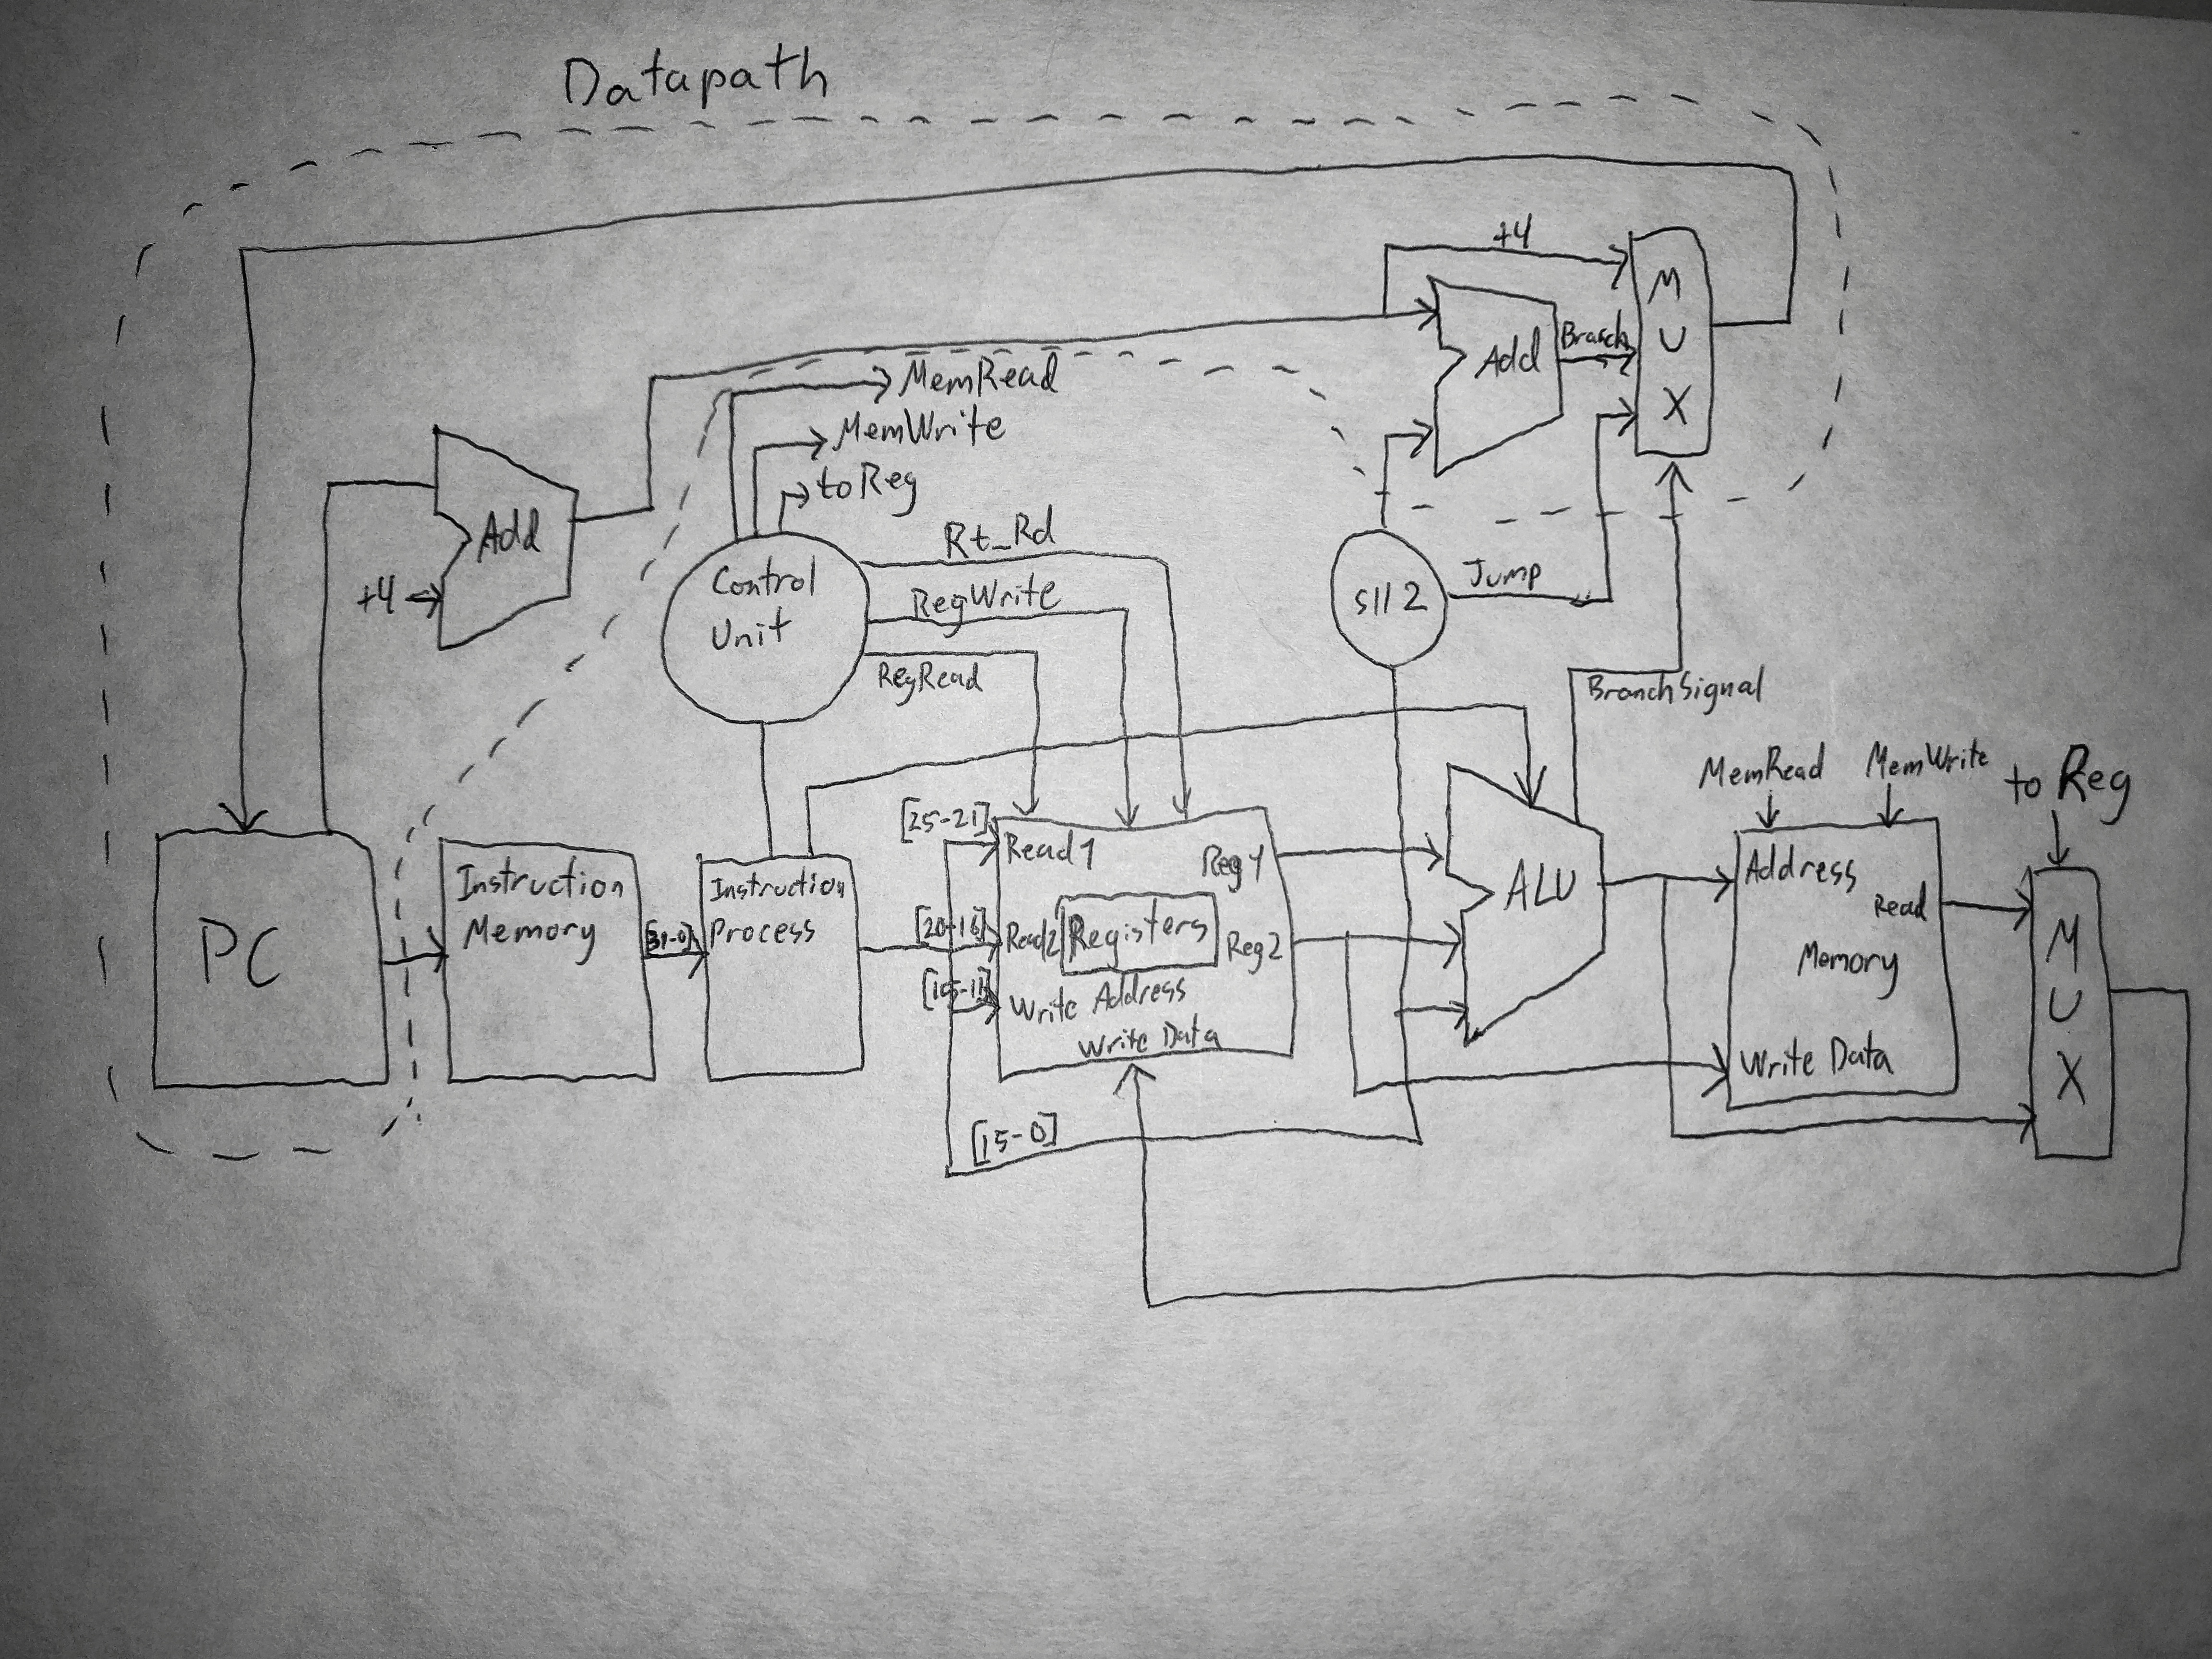
\includegraphics[width=14cm]{./datapath.jpg}

\section{Evaluation}
The procesor was implemented with $display$ commands throughout the modules to make sure each module was executing the right instructions when it needed to. For example: when a instruction was decided on, the ALU would display what instruction it would be. Another example is the InstructionProcess module displaying the different parts of the instruction. After running the three required programs, we can say that the processor is running correctly from the output files that each one generated.



\section{Conclusions}
The procesor was able to execute all proposed instructions sucesfully. The three programs that were created were able to run without flaw. The first one executed all instructions in the first and second column of the table in section 1, the second all instructions in the third column and the third program the instructions in the fourth column. Because of the $display$ commands and the output files we can be sure that the processor is running correctly. It should be noted that our processor includes an extra module, not included in procesors, mostly for ease of implementation. This is the InstructionProcess module, it could be included in the InstructionMemory module. Some other modules also include multiplexers in them, this was done to simplify the reading of the program making the main functional modules of the processor connected to each other with not much hardware between them.

\section{Comments}
The implementation of the processor was pretty straight forward, the process was divided into each independent module and the processor was built as each piece was completed. The main difficulty encountered was the wire management. Knowing where each wire had to go became mind-boggling at a point due to the amount of wires being used. The other main difficulty was trying to determine what signals would activate each always block in the modules, missing one variable would mean the instruction that was fetched would not run correctly, this was fixed with the help of the $display$ commands in the debugging process as they would show how our data was moving in the processor and we could pinpoint the exact parts where the error was ocurring.


\end{document}
